\documentclass{article}
\usepackage{graphicx} % Required for inserting images

\title{Proiect LFT \\
Translator JSON to XML}
\date{May 2023}

\begin{document}

\maketitle
\section{Coechipieri}
\textit{Moldovan Flavia - Adriana} \\
\textit{Neacă Radu - Sabin}\\
\textit{David Dan Ioan}\\
\section{Introduction}
Proiectul de față realizează un translator XML, JSON. Primește ca input un fișier JSON și realizază conversia în fișier XML. \\
\section{Descriere teoretica}
Din punct  de vedere teoretic, pentru rezolvarea problemei avem nevoie de 2 fișiere : un fișier LEX și un fișier YACC. \\
Fișierul LEX este responsabil pentru analiza lexicală. Aici definim reguli care ajută la identificarea token-urilor în codul XML. Aceste reguli specifică de fapt tipurile de caractere și cum să fie ele recunoscute.\\
Fisierul YACC este responsabil pentru analiza sintactica. Aici definim productiile gramatici pentru analiza sintactica a XML-ului. Acestea specifica structura corecta a XML-ului si descriu cum sa fie construit arborele de parsare.

\section{Detalii de implementare}
Concret, în proiect avem următoarele token-uri: OPB (paranteza dreapta deschisa), CLB (paranteza dreapta inchisa), DOT (punct), CMM (virgula), OPENBRACES (acolada deschisa), etc... \\
Mai departe, Se includ fișierele antet necesare, cum ar fi stdio.h, string.h și stdlib.h. Apoi se declară prototipuri de funcții pentru yyerror și yylex, variabile externe yyin (pointer la fișierul de intrare) și linenum (contor pentru numărul de linii), un pointer la fișier out pentru a scrie ieșirea într-un fișier,o variabilă întreagă t pentru a urmări tipul de valori (0 pentru șir, 1 pentru întreg, 2 pentru zecimal, 3 pentru boolean).\\
Definim o structură node pentru a reprezenta un nod al unei liste înlănțuite pentru numele variabilelor. Structura conține un câmp name care reprezintă numele variabilei și un pointer next către următorul nod. \\
Partea cea mai importanta este cea in care definim regulile gramaticii și acțiunile corespunzătoare.
Regula program reprezintă punctul de pornire al programului și definește structura întregului program.
Regula body reprezintă corpul programului și gestionează atribuirea variabilelor și valorilor.
Regula val reprezintă diferitele valori posibile care pot fi atribuite variabilelor, inclusiv tablouri, corpuri, valori true/false și identificatori.
Regula x gestionează identificatorii de variabile și tipurile acestora.
Regulile arr și elements gestionează tablourile și elementele acestora.

\section{Screenshots}\\
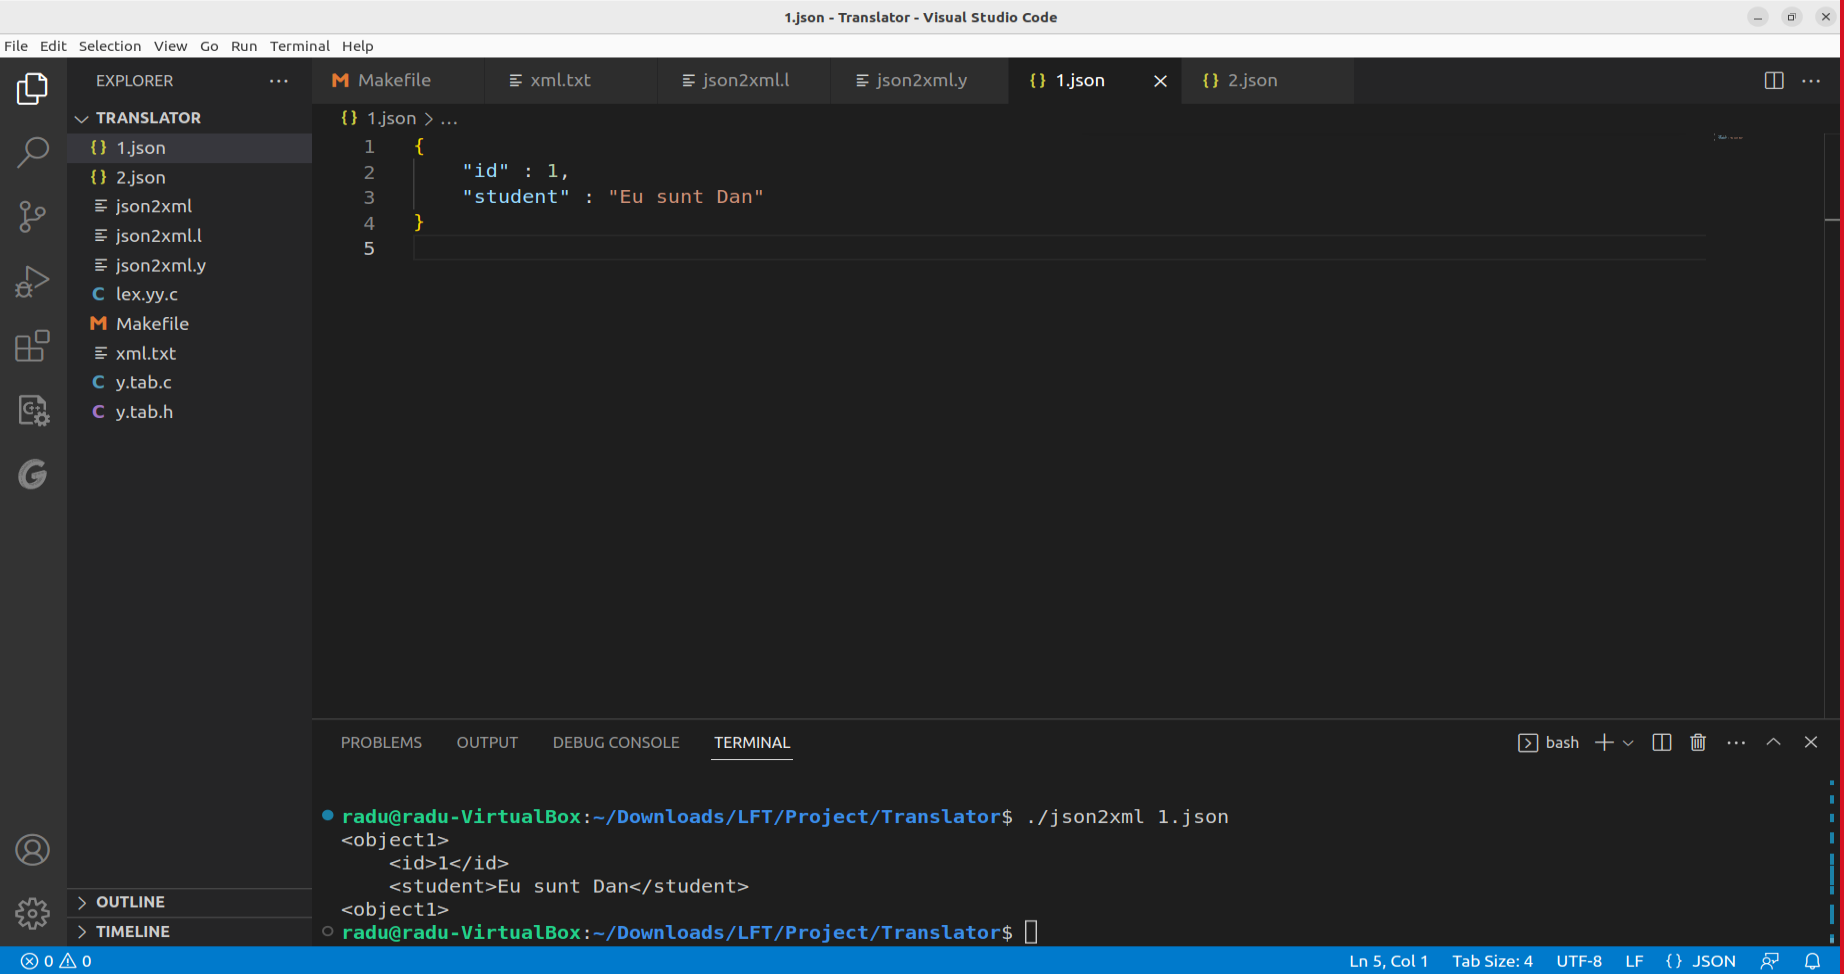
\includegraphics[width=\linewidth]{ss1.png}\\
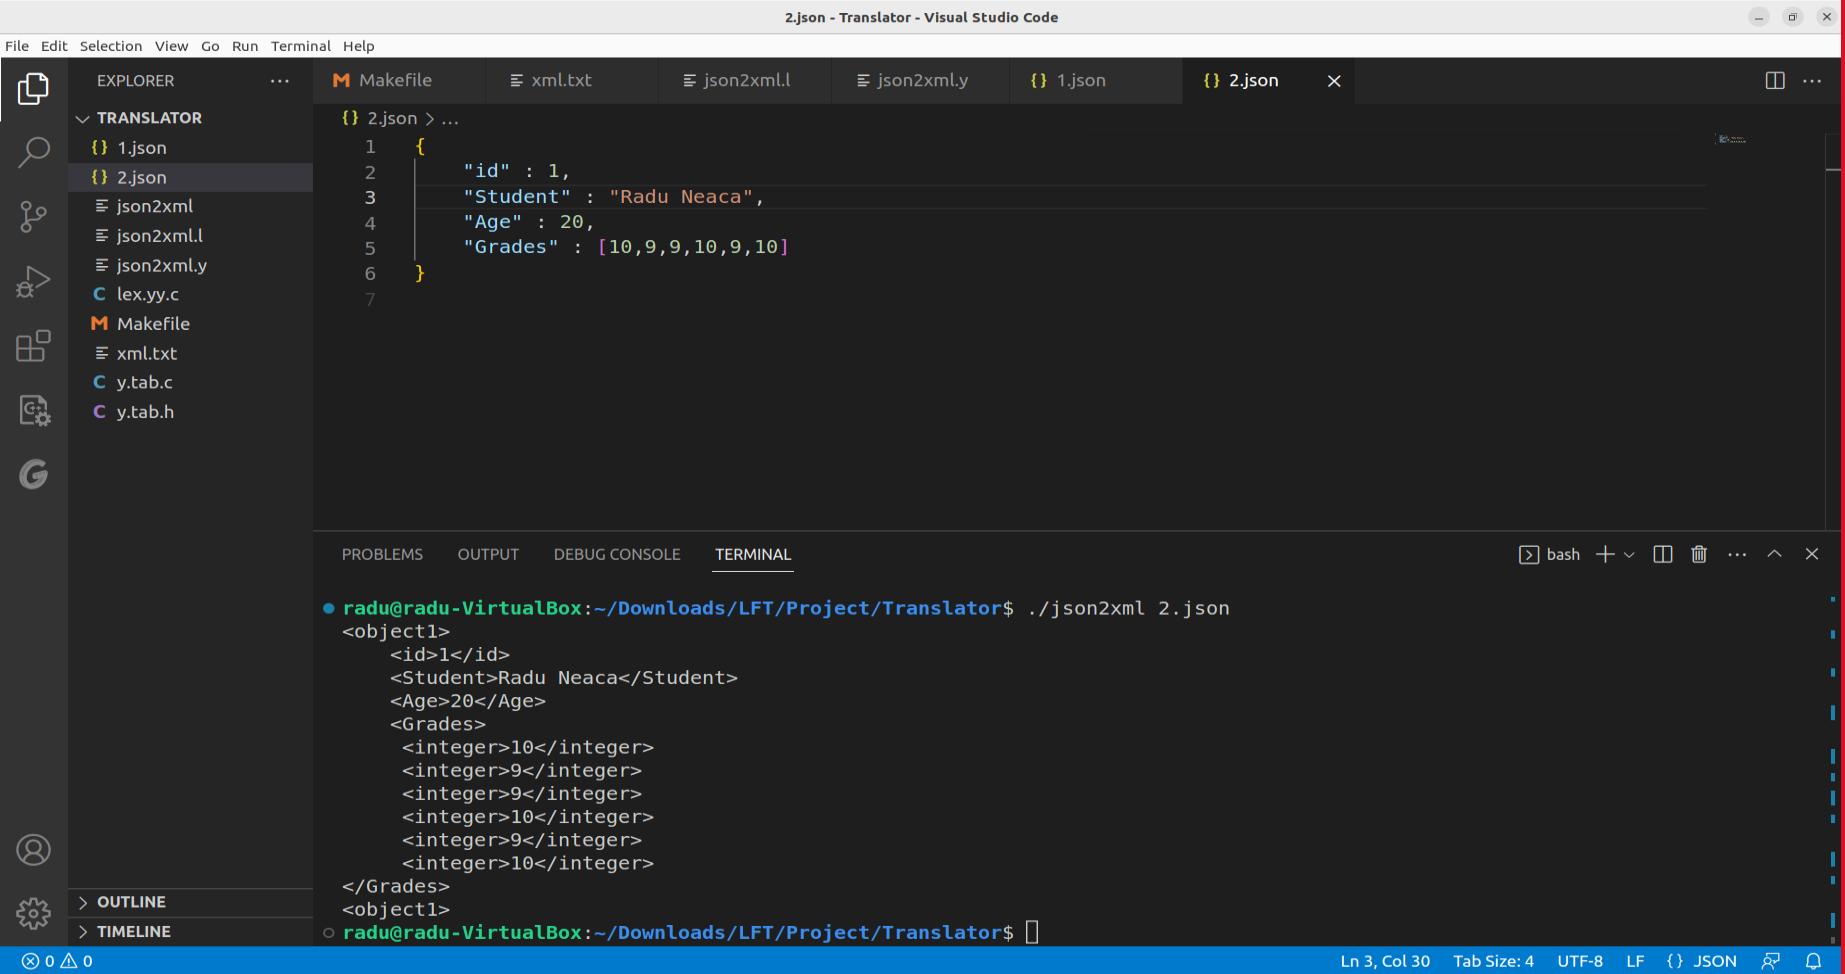
\includegraphics[width=\linewidth]{ss2.png}\\
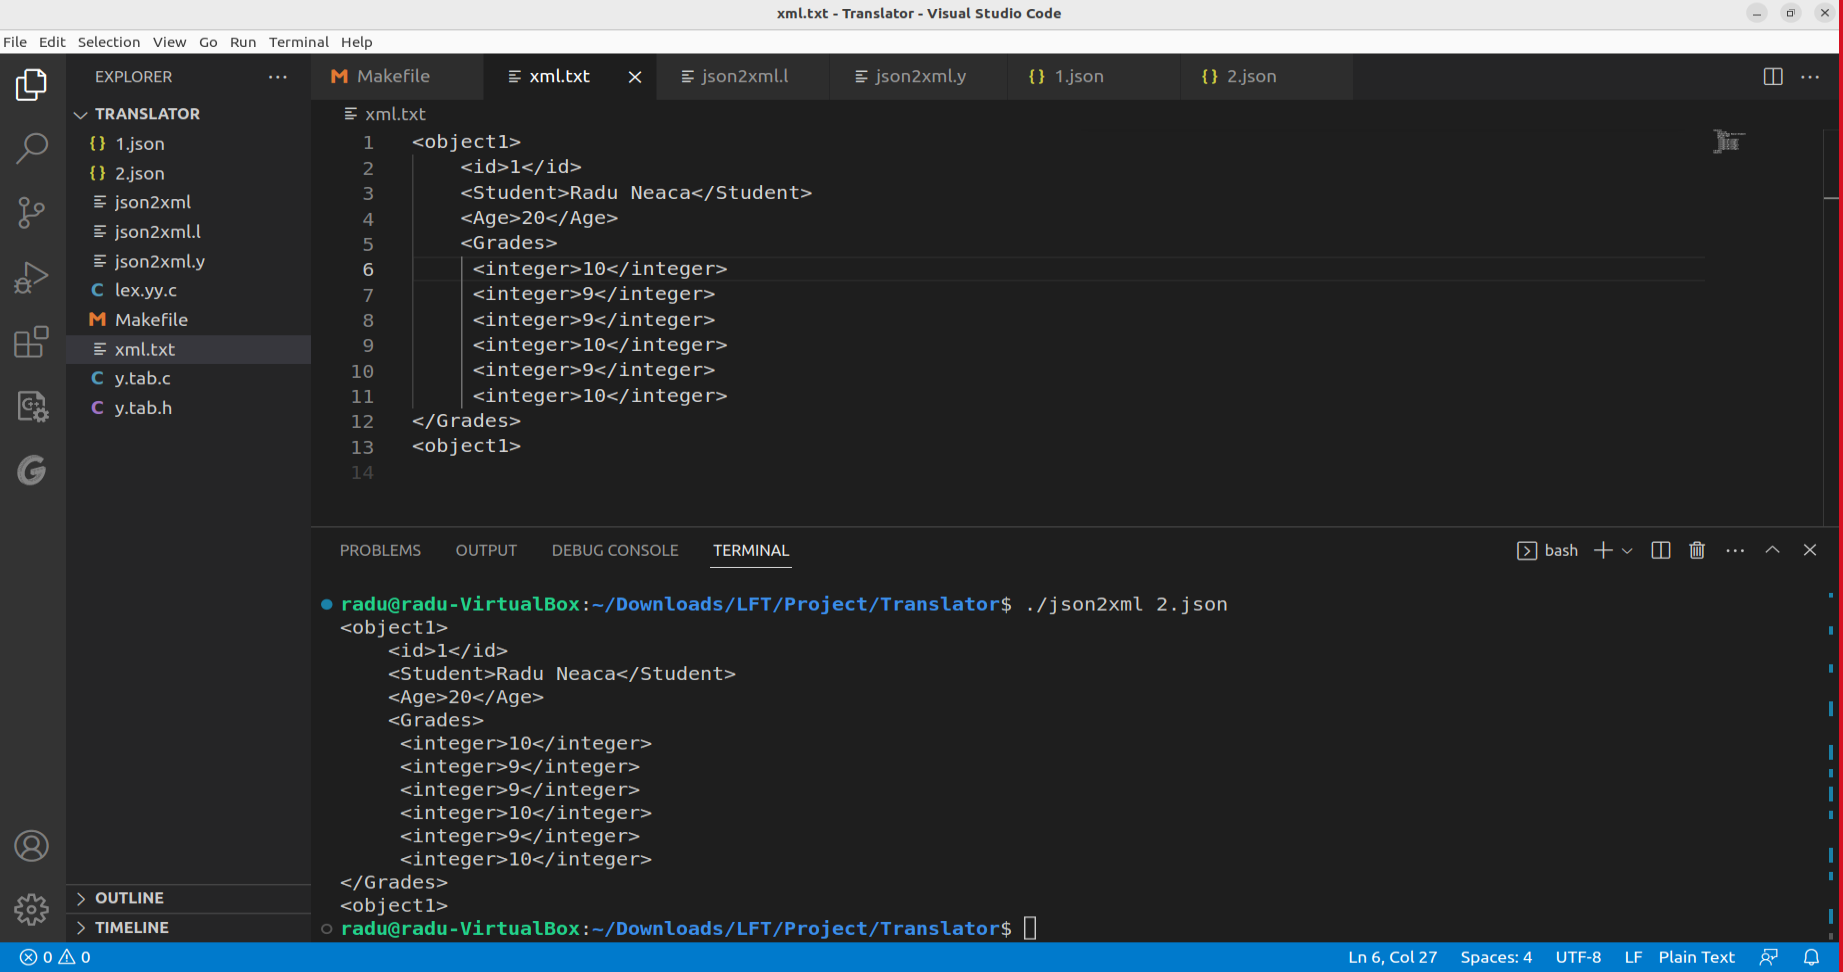
\includegraphics[width=\linewidth]{ss3.png}\\
\section{Link to Github}
\url{https://github.com/Flaviaaa123/LFT} \\
\end{document}
